\documentclass{article}
\usepackage[utf8]{inputenc}
\usepackage{polski}
\usepackage{graphicx}
\usepackage{tikz}
\usetikzlibrary{arrows}
\graphicspath{ {.} }

\usepackage{amssymb, amsmath, amsfonts, amsthm, cite, mathtools, enumerate, rotating, hyperref}
\newcommand \eq[1]{\begin{equation} \begin{split}  #1 \end{split} \end{equation}}


\makeatletter
\def\@seccntformat#1{%
  \expandafter\ifx\csname c@#1\endcsname\c@section\else
  \csname the#1\endcsname\quad
  \fi}
\makeatother

\title{Ćwiczenia 1 SI}
\date{24.03.2020}
\author{Maurycy Borkowski}
\begin{document}
\maketitle

\section{4}
a)\\
\includegraphics{labirynt2}
\\\\
b)
\\
$b = 5$ \\ będziemy się poruszać na wszystkie możliwe pola możliwe dla agenta. Gdy spotka się on z wrogem 'wyrzucamy' z kolejki'. W stanie trzymamy pole naszego agenta oraz czas po to by liczyć później pozycje wrogów.

\section{2,3}
Liczę wszystkie możliwe kombinacje poszczególnych figur u blotkarza i figuranta.\\
Wymnażam układy u blotkarza razy wszystkie gorsze układy figuranta. Te iloczyny sumuję i dzielę przez iloczyn wszystkich rąk.\\
8.452879986493432
\section{5}
Przestrzenie stanów:
\\a)  $db^K$ gdzie $d$ to najdłuższa ścieżka w grafie
\\b)  $d{(b+1)}^K$
\\Efektywniejsze rozwiązanie do b)\\
Tworzymy graf silnie spójnych składowych. W nim sprawdzamy czy dla każdych SSS, w których są przyjaciele czy LCA tych dwóch wierzchołków jest jednym z nich. Jeżeli istnieje para wierzchołków nie spełniająca tego warunku nie istnieje rozwiązanie.
\\
Teraz wszystkich przyjaciół kierujemy do najniższej (w sensie drzewa) niepustej SSS.
\section{6}
$$
h = max(odl_{Man}(king_b, king_c),0) + banda_{uciekajacy} + max(banda_{goniacy}-3,0)
$$
gdzie banda to odległość do najbliższej krawędzi.
\\
W drugim przypadku minimum z h gdy biały goni a czarny ucieka i odwrotnie.

\section{7}
Z warunku spójności mamy:
$$
h(s_2) + cost(s_1,s_2) \geq h(s_1)
$$
$$
cost(s_1,s_2) \geq h(s_1) - h(s_2)
$$
Koszt dojścia z $s_1$ to stanu końcowego możemy zapisać jako sumę:
$$
C = \sum_{i = 1}^{n} cost(s_{i-1},s_i) \geq \sum_{i = 2}^{n} h(s_{i-1}) - h(s_{i}) = h(s_1) - h(s_n) = h(s_1) - 0 = h(s_1)
$$

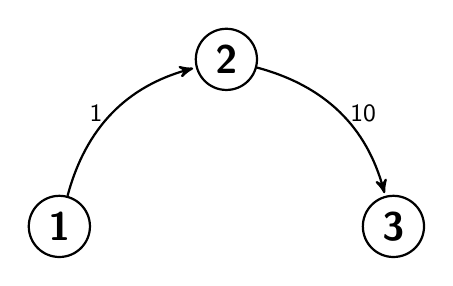
\begin{tikzpicture}[->,>=stealth',shorten >=1pt,auto,node distance=3cm,
                    thick,main node/.style={circle,draw,font=\sffamily\Large\bfseries}]
  \node[main node] (1) {2};
  \node[main node] (2) [below left of=1] {1};
  \node[main node] (4) [below right of=1] {3};

  \path[every node/.style={font=\sffamily\small}]
    (1)
    (2) edge [bend left] node[left] {1} (1)
    (1) edge [bend left] node[right] {10} (4);
\end{tikzpicture}
$h(1) = 10, h(2) = 1$ Łatwo zauważyć, że heurystyka jest optymistyczna, ale $h(2) + cost(1,2) = 2 < 10 = h(1) $

\section{8}
Oznaczmy, przez $v_1$ i $v_2$ punkty stany docelowe w naszym drzewie. $v_1$ stan, który zwrócił $A^*$.\\
Pokażę, że $g(v_1) \leq g(v_2)$:
\\Niech $v$ będzie $LCA(v_1,v_2)$ a $v^{\prime}$ pierwszym nierozwiniętym wierzchołkiem na ścieżce do $v_2$.
\begin{proof}
Z definicji $A^*$ (bo go nie rozwinęliśmy):
$$
f(v_1) \leq f(v^\prime)
$$
$$
g(v_1) + h(v_1) \leq g(v^\prime) + h(v^\prime)
$$
$$
g(v_1) + 0 \leq g(v^\prime) + h(v^\prime)
$$
$C(w)$ koszt dotarcia do najbliższego stanu docleowego z $w$. Z optymalności $h$ oraz jedyności ścieżki\\
$$
g(v^\prime) + h(v^\prime) \leq g(v^\prime) + C(v^\prime) = g(v_2)
$$
\end{proof}
\end{document}

% Nieużywane Kursory